\chapter[Metodoloxía]{
  \label{chp:metodoloxia}
  Metodoloxía
}
\minitoc
\newpage

A metodoloxía de traballo baseouse nos principios das \textbf{metodoloxías áxiles} aplicando, concretamente, aquelas prácticas e técnicas de \textbf{\say{Extreme Programming}} (XP) adaptables ao traballo individual. Destacarase, pola súa especificidade, o uso da técnica de \say{Test Driven Development} (TDD) nalgunhas partes do desenvolvemento.

\section{Principios das metodoloxías áxiles}

Considéranse áxiles aquelas metodoloxías motivadas por unha serie de valores e que respectan unha serie principios, ambos recollidos no \say{manifesto áxil} do ano 2001 \cite{axiles}. Eses valores son:

\begin{itemize}
	\item \textbf{Os individuos e súa interacción} valórase máis que as ferramentas e os procesos.
	\item \textbf{O correcto funcionamento do software} valórase máis que a documentación extensiva.
	\item \textbf{A colaboración co cliente} valórase máis que a negociación contractual.
	\item \textbf{A resposta ante o cambio} valórase máis que o seguimento dun plan.
\end{itemize}

Que se traducen nos chamados \textbf{\say{Doce principios do Software Áxil}}:

\begin{enumerate}
\item A nosa maior prioridade é satisfacer ao cliente
mediante a entrega temperá e continua de software
con valor.

\item Aceptamos que os requirimentos cambien, incluso en etapas 
tardías do desenvolvemento. Os procesos Áxiles aproveitan
o cambio para proporcionar vantaxe competitiva ao 
cliente.

\item Entregamos software funcional frecuentemente, entre dúas
semanas e dous meses, con preferencia ao período de 
tempo máis corto posible.

\item Os responsables de negocio e os desenvolvedores
traballamos xuntos de forma cotiá durante todo
o proxecto.

\item Os proxectos desenvólvense en torno a individuos 
motivados. Hai que darlles o entorno e o apoio que 
necesitan, e confiarlles a execución do traballo. 

\item O método máis eficiente e efectivo de comunicar 
información ao equipo de desenvolvemento e entre os seus 
membros é a conversación cara a cara.

\item O software funcionando é a medida principal de 
progreso.

\item Os procesos Áxiles promoven o desenvolvemento 
sostible. Los promotores, desenvolvedores e usuarios
debemos ser capaces de manter un ritmo constante 
de forma indefinida.

\item A atención continua á excelencia técnica e ao 
bo deseño mellora a Axilidade.

\item A simplicidade, a arte de maximizar a cantidade de
traballo non realizado, é esencial.

\item As mellores arquitecturas, requirimentos e deseños
emerxen de equipos auto-organizados.

\item A intervalos regulares o equipo reflexiona sobre
como ser máis efectivo para a continuación axustar e
perfeccionar o seu comportamento en consecuencia.
\end{enumerate}


\section{Extreme Programming}

Extreme Programming (XP), ou Programación Extrema, é un estilo de desenvolvemento de software que promove unha serie de valores de cara ao traballo en equipo e unha serie de técnicas que supoñen unha simplificación e unha alternativa flexible en contraposición a outras metodoloxías máis tradicionais coma, por exemplo, o \say{desenvolvemento en fervenza}.

Eses valores enuméranse coma\cite{xp}: 

\begin{itemize}
	\item \textbf{Comunicación:} Tanto entre programadores coma co cliente.
	\item \textbf{Simplicidade:} Que o código sexa lexible e a documentación concisa.
	\item \textbf{Retroalimentación:} Realizar iteracións curtas para obter opinións rápidas sobre os progresos.
	\item \textbf{Coraxe:} Aceptar que a aparición de novos requirimentos é natural e poden redefinir o deseño.
	\item \textbf{Respecto:} Estrutura horizontal do equipo de desenvolvemento.
\end{itemize}


A posta en práctica dos anteriores valores lévanos a unha metodoloxía de traballo baseada no contacto continuo co cliente para poder obter correccións e ideas novas (retroalimentación). Isto acádase mediante ciclos curtos de desenvolvemento, ao final dos cales volveremos reunirnos co usuario obxectivo e o ciclo volve a comezar. 

Referímonos a estes ciclos coma \textbf{iteracións} Poden ser tomadas coma unha planificación do traballo a curto prazo a entender non coma unha improvisación, senón coma unha peza dun plan global suxeito á evolución do proxecto. 

A esas \say{ideas novas} que aparecen en cada iteración  chamámoslles \textbf{historias de usuario}. Unha historia de usuario consiste nunha frase concisa onde o usuario obxectivo expresa unha necesidade que ha de ser cuberta polo sistema.

Debido á aceptación de que os sucesivos cambios no deseño son inevitables (coraxe) e que a refactorización de código é algo necesario para asegurar a súa cualidade (simplicidade), faise necesaria a automatización de probas e a utilización dun control de versións.

A metodoloxía XP ten unha serie de características aplicables ao traballo en equipo que non se levaron a cabo neste proxecto: A programación por parellas, a revisión de código entre desenvolvedores ou a división do traballo en función da especialización do persoal (Testers, deseñadores de interacción, directores do proxecto, programadores...)

\subsubsection{Aporte da metodoloxía ao proxecto}

Ao ser este un Proxecto de Final de Carreira, as reunións co cliente substituíronse por \textbf{reunións co director do proxecto de periodicidade quincenal}. Nelas, revisábanse os progreso e xurdían novas historias de usuario (ou se actualizaban as vellas). Grazas a este modo de traballo conseguíronse identificar varios \textbf{requirimentos non valorados a priori} coma, por exemplo, a necesidade de establecer roles de usuario. 

Para afondar individualmente en cada iteración, ver o capítulo \ref{chp:plan} sobre a planificación.


\section{Test Driven Development}

Test Driven Development (TDD) é unha técnica utilizada nas metodoloxías áxiles de desenvolvemento que segue a filosofía \textbf{probar primeiro}. Esta baséase na conversión dos requirimentos en probas antes da propia existencia de código que as avale. Isto obriga ao desenvolvedor a pensar nos requirimentos con detemento, identificar de antemán os posibles fallos e aumentar o alcance da validación de datos. Unha vez o test está definido, pasarase a implementación da funcionalidade posta a proba. De pasar a proba, repítese co seguinte requirimento. Este ciclo pode verse no esquema da figura \ref{fig:tdd}.

\begin{figure}[h]
	\centering
	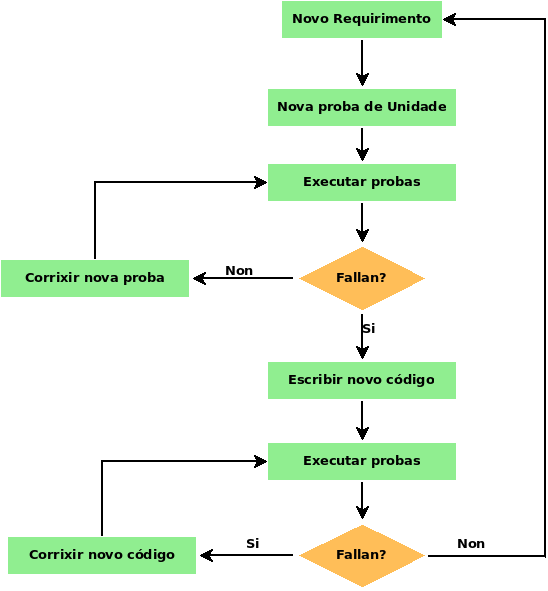
\includegraphics[scale=0.55,keepaspectratio=true]{./images/TDD.png}
	\caption{Diagrama do ciclo de desenvolvemento coa metodoloxía TDD.}
	\label{fig:tdd}
\end{figure}

Existen distintas estratexias á hora de seguir o citado ciclo \cite{tdd} que se poden utilizar en función das características do requirimento:

\begin{itemize}
	\item \textbf{Fake it ('til you make it):} Ou \say{falséao (ata que o fagas)}. Baséase en escribir primeiro un método falso que devolva un valor constante que satisfaga o test. A partir de aí, ilo modificando aos poucos sempre vixiando que o test sexa positivo até que o método estea completo. Esta práctica é moi complexa de utilizar se os métodos son grandes, polo que pode ser unha boa forma de forzar a división, algo desexable para a cualidade do código.
	
	\item \textbf{Triangulación:} Consiste en facer as mesmas comprobación 2 ou máis veces con parámetros distintos dos que esperemos unha saída distinta coa fin de abstraer a función a implementar a raíz dos resultados esperados. Esta implementación é útil para evitar os parámetros superfluos que poidan aparecer nas funcións complexas.
	
	\item \textbf{Implementación Obvia:} Para as funcionalidades sinxelas, non paga a pena utilizar estratexias de abstracción. Podemos simplemente implementar o método e agardar a que o test non falle. Queda a discreción do desenvolvedor definir que funcións son sinxelas e complexas.
	
	\item \textbf{Un a Moitos:} No caso daqueles métodos que actúan sobre unha pluralidade de obxectos, esta estratexia avoga por dividir o requirimento en dous: Habería que validar primeiro o un método que actuaría sobre unicamente un obxecto e, a continuación, validar que se execute sobre dita colección.  

\end{itemize}


Neste proxecto, seguiuse maioritariamente a terceira estratexia da anterior lista por resultar máis intuitiva para o traballo a realizar.

\subsubsection{Aporte da técnica ao proxecto}

Considerouse a utilización de TDD durante a \textbf{implementación do modelo de datos} (ver primeiras iteracións no capítulo \ref{chp:plan}), ao predicirse que sería un código moi sensible aos cambios podería dar pé a regresións. Tamén axudou ao análise de requirimentos ao forzarnos a pensar nos resultados posibles de cada método de antemán.

O uso de TDD forzou a temperá implementación de probas automatizadas, que se poden ver detalladas no capítulo \ref{chp:test} sobre as probas do sistema.


